\documentclass[aspectratio=169]{beamer}
\usetheme{Madrid}
\usecolortheme{default}

% Packages
\usepackage{amsmath}
\usepackage{amsfonts}
\usepackage{amssymb}
\usepackage{graphicx}
\usepackage{pgfplots}
\usepackage{algorithm}
\usepackage{algpseudocode}
\usepackage{booktabs}
\usepackage{xcolor}
\usepackage{tikz}
\usetikzlibrary{shapes.geometric}
\usepackage{pgfplots}
\pgfplotsset{compat=1.18}
\usepackage[utf8]{inputenc}
\usepackage{multimedia}
% Required package
\usepackage{animate}

% Enable graphics extensions
\DeclareGraphicsExtensions{.pdf,.png,.jpg,.jpeg,.gif,.svg}

% Custom colors
\definecolor{juliagreen}{RGB}{56, 152, 38}
\definecolor{juliablue}{RGB}{64, 99, 216}
\definecolor{juliared}{RGB}{213, 99, 92}
\definecolor{juliapurple}{RGB}{149, 88, 178}

% Title page information
\title[IPA Framework]{The Information Propagation Framework}

\begin{document}

% Title slide
\begin{frame}
\titlepage
\end{frame}


\begin{frame}{The Information Propagation Framework}
\begin{center}
\includegraphics[height=0.5\textheight]{IPA.png}
\end{center}
\begin{block}{}
A \textcolor{juliagreen}{\textbf{Julia-based}} framework for network reliability analysis and information propagation that offers a collection of algorithms for analysing how information such as failures, time, cost, capacity or other factors propagate through complex networks that can be modelled as Directed Acyclic Graphs (DAGs).
\end{block}
\end{frame}

\begin{frame}{The Core Idea}
\textbf{The Framework is based on two fundamental concepts:}
\begin{enumerate}
\item \textbf{\textcolor{juliablue}{Topological Sorting of DAGs}}
\begin{itemize}
\item Provides the fixed processing order of nodes in the network as Iteration sets
\item Guarantees dependencies are resolved before dependent nodes
\item Natural parallelisation boundaries
\end{itemize}
\item \textbf{\textcolor{juliagreen}{Iterative Message Passing}}
\begin{itemize}
\item Information starts from sources to sinks in ordered layers
\item Information is computed directly from all dependencies 
\end{itemize}
\end{enumerate}

\vspace{0.2cm}
\begin{center}
\includegraphics[height=0.4\textheight]{msgpage.png}
\end{center}

\end{frame}

\begin{frame}{Why DAGs? The Mathematical Advantage}
\begin{columns}
\begin{column}{0.6\textwidth}
\textbf{Directed Acyclic Graphs provide:}

\begin{itemize}
\item \textbf{Computational Guarantee:} No cycles = No infinite loops
\item \textbf{Optimal Substructure:} Local solutions build to global optimum  
\item \textbf{Natural Parallelization:} Nodes in same topological layer are independent
\item \textbf{Exact Solutions:} No need for iterative convergence
\end{itemize}

\vspace{0.3cm}

\textbf{Mathematical Complexity For Most Algos:}
\begin{align}
\text{Time Complexity} &= O(V + E) \\
\text{Space Complexity} &= O(V + E) \\
\text{Parallelization} &= O(\log V)
\end{align}
\end{column}

\begin{column}{0.4\textwidth}
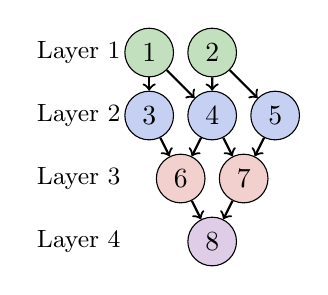
\begin{tikzpicture}[scale=0.8]
% Nodes
\node[circle, draw, fill=juliagreen!30] (1) at (0,3) {1};
\node[circle, draw, fill=juliagreen!30] (2) at (1,3) {2};
\node[circle, draw, fill=juliablue!30] (3) at (0,2) {3};
\node[circle, draw, fill=juliablue!30] (4) at (1,2) {4};
\node[circle, draw, fill=juliablue!30] (5) at (2,2) {5};
\node[circle, draw, fill=juliared!30] (6) at (0.5,1) {6};
\node[circle, draw, fill=juliared!30] (7) at (1.5,1) {7};
\node[circle, draw, fill=juliapurple!30] (8) at (1,0) {8};

% Edges
\draw[->, thick] (1) -- (3);
\draw[->, thick] (1) -- (4);
\draw[->, thick] (2) -- (4);
\draw[->, thick] (2) -- (5);
\draw[->, thick] (3) -- (6);
\draw[->, thick] (4) -- (6);
\draw[->, thick] (4) -- (7);
\draw[->, thick] (5) -- (7);
\draw[->, thick] (6) -- (8);
\draw[->, thick] (7) -- (8);

% Layer labels
\node[left] at (-0.3,3) {\small Layer 1};
\node[left] at (-0.3,2) {\small Layer 2};
\node[left] at (-0.3,1) {\small Layer 3};
\node[left] at (-0.3,0) {\small Layer 4};
\end{tikzpicture}

\small \textit{Topological layers enable parallel processing within each level}
\end{column}
\end{columns}
\end{frame}

\begin{frame}{The Complete IPA Toolkit - From Graph to Insights}
\begin{center}
\includegraphics[height=0.83\textheight]{ipa_bigpicture.png}
\end{center}
\end{frame}

\begin{frame}{\textcolor{juliagreen}{Input Processing Layer-  Preprocessing Module}}
\textbf{Setting the Stage for Network Analysis}

\vspace{0.2cm}

\begin{columns}
\begin{column}{0.5\textwidth}
\begin{block}{\textcolor{juliagreen}{GenerateGraphModule.jl}}
\small
\begin{itemize}
\item Infrastructure-style DAG generation
\item Realistic network topologies  
\item Configurable parameters
\item Multiple output formats
\end{itemize}
\end{block}
\end{column}
\begin{column}{0.5\textwidth}
\begin{block}{\textcolor{juliagreen}{UndirectedToDagModule.jl}}
\small
\begin{itemize}
\item Undirected $\rightarrow$ DAG conversion
\item Multi-metric importance scoring
\item Dynamic cycle breaking
\item As much edge retention  as possible
\end{itemize}
\end{block}
\end{column}
\end{columns}

\vspace{0.4cm}

\begin{center}
\textbf{Why These Matter:} We couldn't find enough real DAG structures to test with!
\end{center}
\end{frame}


\begin{frame}{\textcolor{juliagreen}{GenerateGraphModule.jl - Creating Realistic Test Networks}}

\begin{columns}
\begin{column}{0.58\textwidth}
\textbf{Key Features:}
\begin{itemize}
\item \textcolor{juliagreen}{\textbf{Ranked Nodes}} - Sources, processing layers, sinks etc
\item \textcolor{juliagreen}{\textbf{Critical Path Generation}} - Connectivity with skip connections
\item \textcolor{juliagreen}{\textbf{Redundancy Control}} - Configurable backup paths
\item \textcolor{juliagreen}{\textbf{Fork/Join Diamond Patterns}} - Realistic branching and merging.  
\end{itemize}

\vspace{0.3cm}
\textbf{Why This Matters:}
\begin{itemize}
\item Creates realistic test scenarios
\item Tries to mimic real infrastructure networks
\end{itemize}
\end{column}
\begin{column}{0.42\textwidth}
\centering
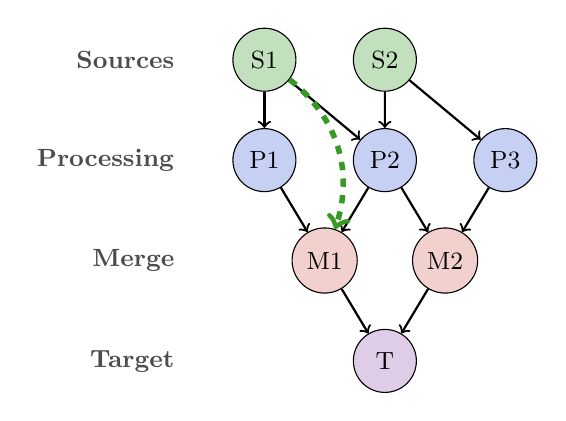
\begin{tikzpicture}[scale=0.85, font=\small]
% Infrastructure-style DAG example with improved spacing
\node[circle, draw, fill=juliagreen!30, minimum size=0.8cm] (s1) at (0,5) {S1};
\node[circle, draw, fill=juliagreen!30, minimum size=0.8cm] (s2) at (1.8,5) {S2};
\node[circle, draw, fill=juliablue!30, minimum size=0.8cm] (p1) at (0,3.5) {P1};
\node[circle, draw, fill=juliablue!30, minimum size=0.8cm] (p2) at (1.8,3.5) {P2};
\node[circle, draw, fill=juliablue!30, minimum size=0.8cm] (p3) at (3.6,3.5) {P3};
\node[circle, draw, fill=juliared!30, minimum size=0.8cm] (m1) at (0.9,2) {M1};
\node[circle, draw, fill=juliared!30, minimum size=0.8cm] (m2) at (2.7,2) {M2};
\node[circle, draw, fill=juliapurple!30, minimum size=0.8cm] (t) at (1.8,0.5) {T};

% Main edges
\draw[->, thick] (s1) -- (p1);
\draw[->, thick] (s1) -- (p2);
\draw[->, thick] (s2) -- (p2);
\draw[->, thick] (s2) -- (p3);
\draw[->, thick] (p1) -- (m1);
\draw[->, thick] (p2) -- (m1);
\draw[->, thick] (p2) -- (m2);
\draw[->, thick] (p3) -- (m2);
\draw[->, thick] (m1) -- (t);
\draw[->, thick] (m2) -- (t);

% Skip connection - more prominent
\draw[->, very thick, dashed, juliagreen, line width=2pt] (s1) to[bend left=35] (m1);

% Layer labels - moved further left
\node[left, font=\small, text=black!70] at (-1.2,5) {\textbf{Sources}};
\node[left, font=\small, text=black!70] at (-1.2,3.5) {\textbf{Processing}};
\node[left, font=\small, text=black!70] at (-1.2,2) {\textbf{Merge}};
\node[left, font=\small, text=black!70] at (-1.2,0.5) {\textbf{Target}};
\end{tikzpicture}

\end{column}
\end{columns}
\end{frame}

\begin{frame}{\textcolor{juliagreen}{UndirectedToDagModule.jl - Graph Conversion}}
\begin{columns}
\begin{column}{0.53\textwidth}
\textbf{Multi-Metric Importance Scoring:}
\begin{itemize}
\item \textcolor{green!70!black}{\textbf{Degree Centrality}} (50\%) - High-traffic nodes get priority for edge retention
\item \textcolor{green!70!black}{\textbf{Eigenvector Centrality}} (30\%) - Considers Overall Network influence, i.e Nodes connected to high traffic nodes matter more
\item \textcolor{green!70!black}{\textbf{Clustering Coefficient}} (20\%) - Aims to preserve Local structure
\end{itemize}
\vspace{0.3cm}
\textbf{Cycle Breaking Flow:}
\begin{enumerate}
\item Edge direction by importance ranking
\item DFS-based cycle detection
\item Remove lowest-importance edges in cycles
\item Validate \& Try again
\end{enumerate}
\end{column}
\begin{column}{0.47\textwidth}
\centering
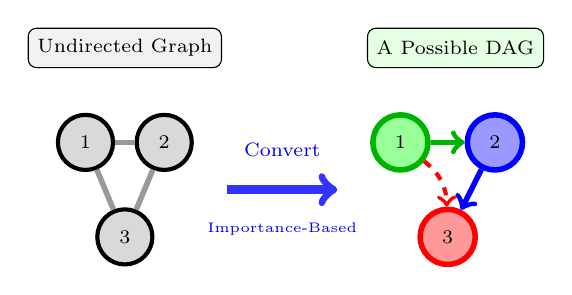
\begin{tikzpicture}[scale=1.0, font=\small]
% Title boxes with better styling
\node[draw, rounded corners=3pt, fill=gray!10, minimum width=2.0cm, minimum height=0.5cm, font=\scriptsize] at (0,4.2) {Undirected Graph};
\node[draw, rounded corners=3pt, fill=green!10, minimum width=2.0cm, minimum height=0.5cm, font=\scriptsize] at (4.2,4.2) {A Possible DAG};

% Before conversion - repositioned for better spacing
\node[circle, draw=black, line width=1.5pt, fill=gray!30, minimum size=0.7cm, font=\scriptsize] (u1) at (-0.5,3.0) {1};
\node[circle, draw=black, line width=1.5pt, fill=gray!30, minimum size=0.7cm, font=\scriptsize] (u2) at (0.5,3.0) {2};
\node[circle, draw=black, line width=1.5pt, fill=gray!30, minimum size=0.7cm, font=\scriptsize] (u3) at (0,1.8) {3};

% Undirected edges - thicker and more visible
\draw[line width=2pt, gray!80] (u1) -- (u2);
\draw[line width=2pt, gray!80] (u2) -- (u3);
\draw[line width=2pt, gray!80] (u3) -- (u1);

% Conversion arrow with styling and text
\draw[->, line width=3pt, blue!80] (1.3,2.4) -- (2.7,2.4);
\node[above, font=\scriptsize, text=blue] at (2.0,2.7) {Convert};
\node[below, font=\tiny, text=blue] at (2.0,2.1) {Importance-Based};

% After conversion - wider spacing for longer arrows
\node[circle, draw=green!70!black, line width=2pt, fill=green!40, minimum size=0.7cm, font=\scriptsize] (d1) at (3.5,3.0) {1};
\node[circle, draw=blue, line width=2pt, fill=blue!40, minimum size=0.7cm, font=\scriptsize] (d2) at (4.7,3.0) {2};
\node[circle, draw=red, line width=2pt, fill=red!40, minimum size=0.7cm, font=\scriptsize] (d3) at (4.1,1.8) {3};

% Directed edges with better visibility and length
\draw[->, line width=2pt, green!70!black] (d1) -- (d2);
\draw[->, line width=2pt, blue] (d2) -- (d3);
\draw[->, line width=1.5pt, red, dashed] (d1) to[bend left=25] (d3);

\end{tikzpicture}
\end{column}
\end{columns}
\end{frame}

\begin{frame}{\textcolor{juliagreen}{Input Processing Module }}

\begin{center}
\textbf{\textcolor{juliagreen}{Compute Once, Use Everywhere - Single graph structure reused across all Modules}}

\includegraphics[width=\textwidth,height=0.85\textheight,keepaspectratio]{input_processing_outputs.png}
\end{center}
\end{frame}

\begin{frame}{\textcolor{juliagreen}{Input Processing Module }}

\begin{center}
\textbf{\textcolor{juliagreen}{Compute Once, Use Everywhere - Single graph structure reused across all Modules}}
\end{center}

\begin{columns}
\begin{column}{0.48\textwidth}
\begin{block}{\textcolor{juliagreen}{Graph Structure}}
\small
\textbf{(edgelist, outgoing\_index, incoming\_index):}
\begin{itemize}
\item O(E) space complexity -so fast lookups
\item Unified representation for all modules
\end{itemize}
\end{block}

\begin{block}{\textcolor{juliagreen}{Topological Structure}}
\small
\textbf{(iteration\_sets, source\_nodes):}
\begin{itemize}
\item Great for parallel processing within levels
\item Guarantees dependency resolution order
\item Natural parallelisation boundaries
\end{itemize}
\end{block}
\end{column}

\begin{column}{0.48\textwidth}
\begin{block}{\textcolor{juliagreen}{Pattern Recognition}}
\small
\textbf{(fork\_nodes, join\_nodes):}
\begin{itemize}
\item Great for diamond pattern analysis
\item Supports redundancy analysis
\end{itemize}
\end{block}

\begin{block}{\textcolor{juliagreen}{Relationship Tracking}}
\small
\textbf{(ancestors, descendants):}
\begin{itemize}
\item Precomputed for O(1) relationship lookups
\item Great for reachability analysis
\item More efficient path finding
\end{itemize}
\end{block}
\end{column}
\end{columns}


\end{frame}

\section{Diamond Classification and Network Decomposition}

\begin{frame}{\textcolor{juliared}{2.1 Diamond Classification Module}}
\centering
\begin{figure}
    \centering
    %\includegraphics{}
     \animategraphics[height=0.6\textheight, loop, autoplay]{1}%frame rate
    {frame_}%path to figures
    {0}%start index
    {5}%end index
\end{figure}

\begin{block}{\textcolor{juliablue}{What are Diamonds?}}
\small
Fork $\rightarrow$ Multiple Paths $\rightarrow$ Join convergence patterns that break independence assumptions in probability calculations
\end{block}
\end{frame}

\begin{frame}{\textcolor{juliared}{Diamond Definition and Mathematical Impact}}
\begin{columns}
\begin{column}{0.55\textwidth}
\textbf{Diamond Structure Components:}
\begin{itemize}
\item \textcolor{juliablue}{\textbf{Fork Node (F):}} Multi-child branching point
\item \textcolor{juliagreen}{\textbf{Join Node (J):}} Multi-parent convergence point
\item \textcolor{juliared}{\textbf{Divergent Paths:}} $\geq$2 distinct paths F$\rightarrow$J
\item \textcolor{juliapurple}{\textbf{Shared Ancestry:}} Common fork ancestor
\end{itemize}

\vspace{0.3cm}
\textbf{Why They Matter:}
\begin{itemize}
\item Break independence assumptions
\item Classical "Noisy-OR" fails
\item Requires exact conditioning on fork states
\item Plus easy parallelisation opportunities
\end{itemize}
\end{column}

\begin{column}{0.45\textwidth}
\centering
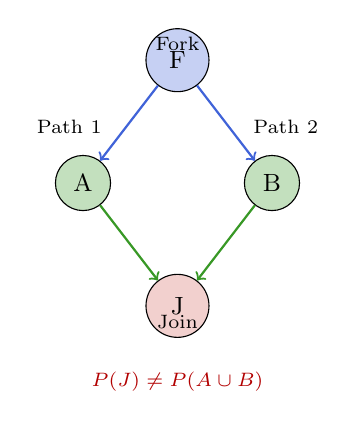
\begin{tikzpicture}[scale=1.2, font=\small]
% Basic diamond structure
\node[circle, draw, fill=juliablue!30, minimum size=0.8cm] (f) at (1.5,3.5) {F};
\node[circle, draw, fill=juliagreen!30, minimum size=0.7cm] (a) at (0.5,2.2) {A};
\node[circle, draw, fill=juliagreen!30, minimum size=0.7cm] (b) at (2.5,2.2) {B};
\node[circle, draw, fill=juliared!30, minimum size=0.8cm] (j) at (1.5,0.9) {J};

% Diamond edges
\draw[->, thick, juliablue] (f) -- (a);
\draw[->, thick, juliablue] (f) -- (b);
\draw[->, thick, juliagreen] (a) -- (j);
\draw[->, thick, juliagreen] (b) -- (j);

% Labels
\node[above, font=\scriptsize] at (f) {Fork};
\node[below, font=\scriptsize] at (j) {Join};
\node[left, font=\scriptsize] at (0.8,2.8) {Path 1};
\node[right, font=\scriptsize] at (2.2,2.8) {Path 2};

% Mathematical notation
\node[below, font=\scriptsize, text=red!70!black] at (1.5,0.3) {$P(J) \neq P(A \cup B)$};
\end{tikzpicture}

\end{column}
\end{columns}
\end{frame}

\begin{frame}{\textcolor{juliared}{Diamond Classification System - 6 Types}}
\begin{columns}
\begin{column}{0.48\textwidth}
\textbf{By Structure Complexity:}
\begin{enumerate}
\item \textcolor{juliagreen}{\textbf{Basic Induced:}} Simple fork-join (1-3 forks)
\item \textcolor{juliablue}{\textbf{Self-influenced:}} Fork connects directly to join
\item \textcolor{juliared}{\textbf{Multi-fork:}} Multiple fork nodes → same join
\end{enumerate}

\vspace{0.3cm}
\textbf{By Advanced Patterns:}
\begin{enumerate}
\setcounter{enumi}{3}
\item \textcolor{juliapurple}{\textbf{Interconnected:}} Diamonds sharing nodes/edges
\item \textcolor{orange}{\textbf{Nested:}} Diamonds within diamonds
\item \textcolor{brown}{\textbf{Chained:}} Sequential diamond structures
\end{enumerate}
\end{column}

\begin{column}{0.52\textwidth}
\textbf{Classification Dimensions:}
\begin{itemize}
\item \textbf{Fork Structure:} Single/Multi/Chained/Self-influence
\item \textbf{Internal Structure:} Simple/Nested/Sequential/Interconnected
\item \textbf{Path Topology:} Parallel/Converging/Branching/Cross-connected
\item \textbf{Join Structure:} Single/Hierarchical/Partial
\item \textbf{External Connectivity:} Isolated/Bridge/Embedded
\end{itemize}


\end{column}
\end{columns}
\end{frame}

\begin{frame}{\textcolor{juliared}{2.2 Network Decomposition Algorithm}}

\begin{columns}
\begin{column}{0.60\textwidth}

\begin{enumerate}
\item \textcolor{juliablue}{\textbf{Shared Ancestor Detection:}} Fork influence mapping
\item \textcolor{juliared}{\textbf{Diamond Group Formation:}} Parent grouping by fork ancestry
\item \textcolor{juliapurple}{\textbf{Subgraph Extraction:}} Complete diamond context
\begin{itemize}
\item All relevant nodes and edges
\item Conditioning nodes
\item Local iteration sets for processing
\item Complete ancestry relationships
\end{itemize}
\end{enumerate}


\end{column}

\begin{column}{0.32\textwidth}
\centering
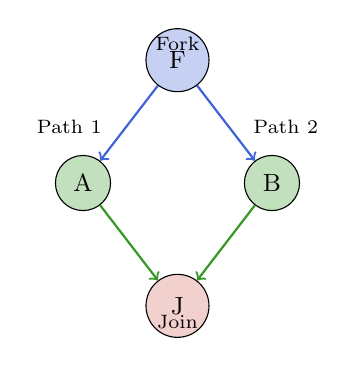
\begin{tikzpicture}[scale=1.2, font=\small]
% Basic diamond structure
\node[circle, draw, fill=juliablue!30, minimum size=0.8cm] (f) at (1.5,3.5) {F};
\node[circle, draw, fill=juliagreen!30, minimum size=0.7cm] (a) at (0.5,2.2) {A};
\node[circle, draw, fill=juliagreen!30, minimum size=0.7cm] (b) at (2.5,2.2) {B};
\node[circle, draw, fill=juliared!30, minimum size=0.8cm] (j) at (1.5,0.9) {J};

% Diamond edges
\draw[->, thick, juliablue] (f) -- (a);
\draw[->, thick, juliablue] (f) -- (b);
\draw[->, thick, juliagreen] (a) -- (j);
\draw[->, thick, juliagreen] (b) -- (j);

% Labels
\node[above, font=\scriptsize] at (f) {Fork};
\node[below, font=\scriptsize] at (j) {Join};
\node[left, font=\scriptsize] at (0.8,2.8) {Path 1};
\node[right, font=\scriptsize] at (2.2,2.8) {Path 2};

\end{tikzpicture}
\end{column}
\end{columns}
\end{frame}

\begin{frame}{\textcolor{juliared}{Diamond Identification Flow}}
\begin{center}
\includegraphics[height=0.9\textheight]{diamond_identification_flow.png}
\end{center}
\end{frame}

\section{Reachability Analysis - Exact Activation Probability}

\section{Reachability Analysis - Exact Activation Probability}

% Frame 1: Problem Introduction
\begin{frame}{\textcolor{juliapurple}{Reachability Analysis }}
\begin{columns}
\begin{column}{0.55\textwidth}
\textbf{The Problem:}
\begin{itemize}
\item Calculate exact probability of node activation from source nodes
\item Handle multiple dependency paths without double-counting
\item Classical "Noisy-OR" overestimates shared ancestor influence
\item Diamond structures break independence assumptions
\end{itemize}

\end{column}

\begin{column}{0.43\textwidth}
\centering
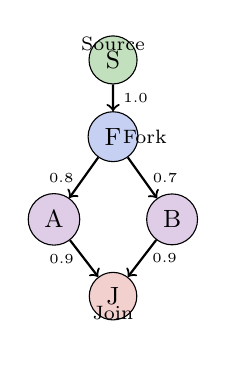
\begin{tikzpicture}[scale=0.75, font=\small]
% Diamond structure: Source → Fork → {A,B} → Join
\node[circle, draw, fill=juliagreen!30, minimum size=0.6cm] (s) at (1.5,4.5) {S};
\node[circle, draw, fill=juliablue!30, minimum size=0.6cm] (f) at (1.5,3.2) {F};
\node[circle, draw, fill=juliapurple!30, minimum size=0.6cm] (a) at (0.5,1.8) {A};
\node[circle, draw, fill=juliapurple!30, minimum size=0.6cm] (b) at (2.5,1.8) {B};
\node[circle, draw, fill=juliared!30, minimum size=0.6cm] (j) at (1.5,0.5) {J};

% Edges with probabilities
\draw[->, thick] (s) -- (f) node[midway, right, font=\tiny] {1.0};
\draw[->, thick] (f) -- (a) node[midway, left, font=\tiny] {0.8};
\draw[->, thick] (f) -- (b) node[midway, right, font=\tiny] {0.7};
\draw[->, thick] (a) -- (j) node[midway, left, font=\tiny] {0.9};
\draw[->, thick] (b) -- (j) node[midway, right, font=\tiny] {0.9};

% Labels
\node[above, font=\scriptsize] at (s) {Source};
\node[right, font=\scriptsize] at (f) {Fork};
\node[below, font=\scriptsize] at (j) {Join};
\node[below, font=\scriptsize, text=red!70!black] at (1.5,-0.1) {};
\end{tikzpicture}

\end{column}
\end{columns}
\end{frame}

% Frame 1b: Problem Introduction
\begin{frame}{\textcolor{juliapurple}{Reachability Analysis - The Diamond Problem}}
\begin{columns}
\begin{column}{0.55\textwidth}
\textbf{The Challenge:}
Simple Noisy-OR combination overestimates when shared dependencies

\vspace{0.25cm}
\textbf{Our Solution:}
\begin{itemize}
\item \textcolor{juliagreen}{\textbf{State conditioning}} on fork nodes 
\item \textcolor{juliablue}{\textbf{Inclusion-exclusion}} for overlapping paths
\item \textcolor{juliared}{\textbf{Cutset extraction}} minimizes conditioning complexity
\item \textcolor{juliapurple}{\textbf{Multiple algorithms}} - same math, different probability representations
\end{itemize}
\end{column}

\begin{column}{0.43\textwidth}
\centering
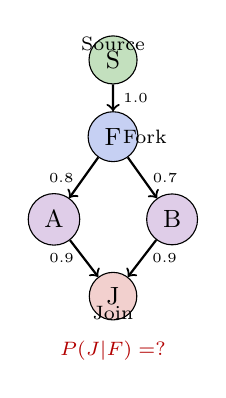
\begin{tikzpicture}[scale=0.75, font=\small]
% Diamond structure: Source → Fork → {A,B} → Join
\node[circle, draw, fill=juliagreen!30, minimum size=0.6cm] (s) at (1.5,4.5) {S};
\node[circle, draw, fill=juliablue!30, minimum size=0.6cm] (f) at (1.5,3.2) {F};
\node[circle, draw, fill=juliapurple!30, minimum size=0.6cm] (a) at (0.5,1.8) {A};
\node[circle, draw, fill=juliapurple!30, minimum size=0.6cm] (b) at (2.5,1.8) {B};
\node[circle, draw, fill=juliared!30, minimum size=0.6cm] (j) at (1.5,0.5) {J};

% Edges with probabilities
\draw[->, thick] (s) -- (f) node[midway, right, font=\tiny] {1.0};
\draw[->, thick] (f) -- (a) node[midway, left, font=\tiny] {0.8};
\draw[->, thick] (f) -- (b) node[midway, right, font=\tiny] {0.7};
\draw[->, thick] (a) -- (j) node[midway, left, font=\tiny] {0.9};
\draw[->, thick] (b) -- (j) node[midway, right, font=\tiny] {0.9};

% Labels
\node[above, font=\scriptsize] at (s) {Source};
\node[right, font=\scriptsize] at (f) {Fork};
\node[below, font=\scriptsize] at (j) {Join};
\node[below, font=\scriptsize, text=red!70!black] at (1.5,-0.1) {$P(J|F) = ?$};
\end{tikzpicture}

\end{column}
\end{columns}
\end{frame}

% Frame 2b: Algorithm Family
\begin{frame}{\textcolor{juliapurple}{Reachability Algorithm Family - 5 Different Approaches}}
\begin{columns}
\begin{column}{0.48\textwidth}
\textbf{\textcolor{juliablue}{Four Exact Algorithms:}}
\begin{itemize}
    \item \textbf{Float:} Single probability values
    \item \textbf{Interval:} $[p_{min}, p_{max}]$ bounds
    \item \textbf{P-box:} Full probability distributions  
    \item \textbf{Path Enumeration:} Alternative exact approach
\end{itemize}

\vspace{0.3cm}
\textbf{\textcolor{juliared}{One Approximate:}}
\begin{itemize}
    \item \textbf{Monte Carlo:} Statistical validation
\end{itemize}
\end{column}

\begin{column}{0.50\textwidth}
\textbf{\textcolor{juliagreen}{Selection Criteria:}}
\begin{itemize}
    \item \textbf{Uncertainty needs:} None, bounds, or full distributions
    \item \textbf{Memory constraints:} 8 bytes to 8KB per probability
    \item \textbf{Speed requirements:} Fast to slow
    \item \textbf{Network size:} Small to unlimited scale
    \item \textbf{Validation needs:} Cross-verification capability
\end{itemize}

\vspace{0.3cm}
\textbf{\textcolor{juliagreen}{Key Point:}}
Same math, different probability representations. Choice depends on the needs for uncertainty and computational constraints.
\end{column}
\end{columns}
\end{frame}

% Frame 3a: Float Algorithm Implementation  
\begin{frame}{\textcolor{juliapurple}{3.1  Reachability Algorithm Family  - Mathematical Implementation}}

\textbf{\textcolor{juliagreen}{Mathematical Implementation:}}
\begin{enumerate}
    \item \textbf{Regular Paths:} Sum parent contributions
    \begin{align}
    P_{\text{parent}}(j) = \sum_{i \in \text{parents}(j)} P(i) \cdot P(i \to j)
    \end{align}
    
    \item \textbf{Multiple Paths:} Apply inclusion-exclusion  
    \begin{align}
    P(A \cup B) = P(A) + P(B) - P(A \cap B)
    \end{align}
    
    \item \textbf{Diamond Conditioning:} Enumerate fork states
    \begin{align}
    P(\text{join}) = \sum_{s \in \{0,1\}^{|F|}} P(\text{join}|s) \cdot P(s)
    \end{align}
    where $F$ = fork nodes, $s$ = binary state vector
    
\end{enumerate}



\end{frame}



% Frame 4: Inputs
% Frame 4a: Input Types  
\begin{frame}{\textcolor{juliapurple}{ Reachability Algorithm Family - Input Types}}
\begin{center}
\textbf{\textcolor{juliapurple}{Same Probability Ops, Different probability representations}}


\end{center}
\begin{columns}
\begin{column}{0.45\textwidth}
\textbf{\textcolor{juliagreen}{Float Reachability (3.1):}}
\begin{itemize}
    \item Standard Float64 values
    \item Example: $P = 0.75$
    \item O(1) Direct arithmetic operations
\end{itemize}

\vspace{0.4cm}
\textbf{\textcolor{juliablue}{Interval Reachability (3.2):}}
\begin{itemize}
    \item Probability bounds: $[p_{min}, p_{max}]$
    \item Example: $P \in [0.6, 0.8]$
    \item O(1) interval arithmetic
\end{itemize}
\end{column}

\begin{column}{0.45\textwidth}
\textbf{\textcolor{juliared}{P-box Reachability (3.3):}}
\begin{itemize}
    \item Full probability distributions (via PBA.jl)
    \item Example: $P \sim \text{Beta}(2,3)$ or $\text{Normal}(\mu, \sigma)$
    \item Complete uncertainty characterisation
    \item Convolution-based arithmetic
\end{itemize}


\end{column}
\end{columns}
\end{frame}

% Frame 4b: Memory and Time Complexity
\begin{frame}{\textcolor{juliapurple}{Reachability Algorithm Family - Memory \& Time Complexity}}
\begin{center}
\begin{tabular}{|l|c|c|c|}
\hline
\textbf{Algorithm} & \textbf{Memory per Prob} & \textbf{Speed} & \textbf{Time Complexity} \\
\hline
\textcolor{juliagreen}{\textbf{Float}} & 8 bytes & Fast & $O(V + E \times 2^d)$ \\
\hline
\textcolor{juliablue}{\textbf{Interval}} & 16 bytes &  Fast & $O(V + E \times 2^d)$ \\
\hline
\textcolor{juliared}{\textbf{P-box}} & ~1.6KB &  Slow & $O(V + E \times 2^d \times n^2)$ \\
\hline
\end{tabular}
\end{center}

\vspace{0.4cm}
\textbf{Key Variables:}
\begin{itemize}
    \item $V$ = nodes, $E$ = edges, $d$ = max fork nodes per diamond
    \item P-box bottleneck: \texttt{PBA.convIndep()} operations
\end{itemize}

\vspace{0.3cm}
\begin{center}
\textbf{\textcolor{juliablue}{Performance Reality:}} P-box convolution transforms O(1) operations into O(n²) around 40,000 operations each
\end{center}
\end{frame}



% Frame 5: Path Enumeration & Monte Carlo
\begin{frame}{\textcolor{juliapurple}{3.4 \& 3.5 Path Enumeration (Exact) \& Monte Carlo (Approximate)}}
\begin{columns}
\begin{column}{0.50\textwidth}
\textbf{\textcolor{juliagreen}{Path Enumeration (Exact):}}
\begin{itemize}
    \item \textbf{Approach:} Find all paths from sources to target
    \item \textbf{Method:} DFS with backtracking
    \item \textbf{Calculation:} Inclusion-exclusion on path sets
    \item \textbf{Exactness:} Mathematically exact
    \item \textbf{Complexity:} Can explode with many paths
    \item \textbf{Use Case:} Alternative verification method, small networks
\end{itemize}


\end{column}

\begin{column}{0.48\textwidth}
\textbf{\textcolor{juliared}{Monte Carlo (Approximate):}}
\begin{itemize}
    \item \textbf{Approach:} Statistical sampling
    \item \textbf{Method:} Sample node/edge states, check reachability
    \item \textbf{Approximation:} Converges to the true value with higher iterations
    \item \textbf{Usage:} Validation and extreme scale networks
\end{itemize}


\end{column}
\end{columns}
\end{frame}

% Frame 6: Complete Comparison
\begin{frame}{\textcolor{juliapurple}{Complete Reachability Family - All 5 Algorithms}}

\begin{center}
\textbf{Four exact algorithms, one approximate - choose based on uncertainty needs, memory constraints, and network size}
\end{center}

\vspace{0.5em}


\begin{center}
\begin{tabular}{|l|c|c|c|}
\hline
\textbf{Algorithm} & \textbf{Exactness} & \textbf{Memory} & \textbf{Speed} \\
\hline
\textcolor{juliagreen}{\textbf{Float}} & Exact & 8 bytes & Very Fast \\
\hline
\textcolor{juliablue}{\textbf{Interval}} & Exact & 16 bytes & Fast \\
\hline
\textcolor{juliared}{\textbf{P-box}} & Exact & 8KB & Slow \\
\hline
\textcolor{juliapurple}{\textbf{Path Enum}} & Exact & Variable & Slow \\
\hline
\textcolor{orange}{\textbf{Monte Carlo}} & Approximate & 8 bytes & Very Slow \\
\hline
\end{tabular}
\end{center}

\end{frame}

% Frame: Future Work on Reachability Family
\begin{frame}{\textcolor{juliapurple}{Future Work (Maybe) - Extending the Reachability Algorithm Family}}
\begin{columns}
\begin{column}{0.48\textwidth}
\textbf{\textcolor{juliagreen}{State-Based Reachability:}}
\begin{itemize}
    \item Multi-state nodes: Working/Failed/Under-Repair
    \item Thread-per-state decomposition for parallelisation
\end{itemize}

\vspace{0.3cm}
\textbf{\textcolor{juliablue}{Temporal Reachability:}}
\begin{itemize}
    \item Time-dependent probability evolution
    \item Event-driven state changes
    \item Cascading failure modelling over time with PBA.jl
\end{itemize}
\end{column}

\begin{column}{0.48\textwidth}
\textbf{\textcolor{juliared}{MTTF/MTTR Type Reliability Analysis:}}
\begin{itemize}
    \item Failure rates: $\lambda = 1/\text{MTTF}$
    \item Repair rates: $\mu = 1/\text{MTTR}$
    \item Cascade multipliers for dependent failures
\end{itemize}

\vspace{0.3cm}
\textbf{\textcolor{juliapurple}{Unified Framework Vision:}}
\begin{itemize}
    \item Same diamond conditioning logic
    \item Extended state spaces beyond binary
    \item Hierarchical parallelisation strategy
\end{itemize}
\end{column}
\end{columns}

\end{frame}





\section{Critical Path Analysis}

\begin{frame}{\textcolor{juliablue}{4. Critical Path Analysis}}

% Top section - full width, horizontal bullet line
\noindent
\textbf{Challenges:} \\
\begin{itemize}
\item \textbf{Find longest/critical path} — “What’s the earliest completion time?” \hfill
\item \textbf{Determine completion time, max cost, bottlenecks} — “What’s the maximum cost path?” \hfill
\item \textbf{Handle multiple criteria (time, cost, risk, capacity)} — “What’s the bottleneck capacity?” \hfill
\item \textbf{Identify critical nodes/edges} — “What’s the worst-case risk accumulation?”
\end{itemize}

\vspace{0.5cm}

% Bottom section - split columns
\begin{columns}
\begin{column}{0.65\textwidth}
\centering
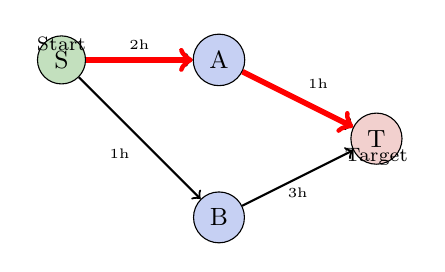
\begin{tikzpicture}[scale=1.0, font=\small]
% Nodes
\node[circle, draw, fill=juliagreen!30, minimum size=0.6cm] (s) at (0,0) {S};
\node[circle, draw, fill=juliablue!30, minimum size=0.6cm] (a) at (2,0) {A};
\node[circle, draw, fill=juliablue!30, minimum size=0.6cm] (b) at (2,-2) {B};
\node[circle, draw, fill=juliared!30, minimum size=0.6cm] (t) at (4,-1) {T};

% Edges
\draw[->, thick] (s) -- (a) node[midway, above, font=\tiny] {2h};
\draw[->, thick] (s) -- (b) node[midway, below left, font=\tiny] {1h};
\draw[->, thick] (a) -- (t) node[midway, above right, font=\tiny] {1h};
\draw[->, thick] (b) -- (t) node[midway, below, font=\tiny] {3h};

% Critical path
\draw[->, very thick, red, line width=2pt] (s) -- (a);
\draw[->, very thick, red, line width=2pt] (a) -- (t);

% Labels
\node[above, font=\scriptsize] at (s) {Start};
\node[below, font=\scriptsize] at (t) {Target};


\end{tikzpicture}
\end{column}

\begin{column}{0.33\textwidth}
\textbf{Node Values:}
\begin{itemize}
\item \textbf{S:} Time=0, Cost=0
\item \textbf{A:} Time=5, Cost=100  
\item \textbf{B:} Time=3, Cost=150
\item \textbf{T:} Time=2, Cost=50
\end{itemize}
\end{column}
\end{columns}
\end{frame}


\begin{frame}{\textcolor{juliablue}{Critical Path Analysis - Mathematical Foundation}}

\textbf{Generalized Algorithm Framework:}
\begin{enumerate}
\item \textbf{Topological Processing:} Use iteration sets for dependency resolution
\item \textbf{Three-Stage Computation:} For each node in topological order:

\begin{align}
\text{Stage 1: } &\text{Propagate}(parent\_value, edge\_value) \\
\text{Stage 2: } &\text{Combine}(propagated\_values) \\
\text{Stage 3: } &\text{Apply Node Processing}(combined\_input, node\_value)
\end{align}
\end{enumerate}

\vspace{0.3cm}
\textbf{Specific Algorithm Instantiations:}

\begin{center}
\begin{tabular}{|l|c|c|c|}
\hline
\textbf{Analysis Type} & \textbf{Combination} & \textbf{Propagation} & \textbf{Node Function} \\
\hline
\textbf{Time Critical Path} & $\max()$ & $parent + edge$ & $input + duration$ \\
\hline
\textbf{Cost Analysis} & $\max()$ & $parent + edge$ & $input + cost$ \\
\hline
\textbf{Bottleneck/Capacity} & $\max()$ & $\min(parent, edge)$ & $\min(input, capacity)$ \\
\hline
\textbf{Risk Analysis} & $\max()$ & $parent + edge$ & $input + risk$ \\
\hline
\end{tabular}
\end{center}

\end{frame}

\begin{frame}{\textcolor{juliablue}{Critical Path Analysis - Input Types and Flexibility}}

\begin{columns}
\begin{column}{0.48\textwidth}
\textbf{\textcolor{juliagreen}{Time Analysis Inputs:}}
\begin{itemize}
\item \texttt{task\_durations}: Duration per node
\item \texttt{edge\_delays}: Dependency delays
\item \texttt{start\_time}: Project start time
\item Multiple time units supported (hours, days, etc.)
\item NonNegativeTime for exact calculations
\end{itemize}

\vspace{0.3cm}
\textbf{\textcolor{juliablue}{Cost Analysis Inputs:}}
\begin{itemize}
\item \texttt{node\_costs}: Processing costs per node
\item \texttt{edge\_costs}: Transmission/setup costs
\item \texttt{start\_cost}: Initial project cost
\end{itemize}
\end{column}

\begin{column}{0.48\textwidth}
\textbf{\textcolor{juliared}{Capacity Analysis Inputs:}}
\begin{itemize}
\item \texttt{node\_capacities}: Processing limits
\item \texttt{edge\_capacities}: Transmission limits
\item \texttt{initial\_capacity}: Source capacity
\end{itemize}

\vspace{0.3cm}
\textbf{\textcolor{juliapurple}{Custom Analysis:}}
\begin{itemize}
\item Define custom combination functions
\item Define custom propagation functions
\item Define custom node processing
\item Support any numeric type
\item Configurable optimization objectives
\end{itemize}
\end{column}
\end{columns}

\vspace{0.3cm}
\begin{center}
\textbf{All \textcolor{juliagreen}{O(V + E)} complexity using iteration sets from Input Module}
\end{center}
\end{frame}

\section{Capacity Analysis}
\begin{frame}{\textcolor{orange}{Capacity Analysis – Overview}}



\vspace{0.4cm}
\textbf{\textcolor{orange}{Supports four capacity analysis types:}}

\vspace{0.3cm}
\begin{itemize}
    \item \textbf{1. Maximum Flow with Processing Limits:} Flow is limited by edge and node capacities.
    \item \textbf{2. Bottleneck (Widest Path) Analysis:} Tracks the narrowest point along the most permissive path.
    \item \textbf{3. Classical Max Flow:} Ignores processing limits at nodes; pure transmission capacity.
    \item \textbf{4. Multi-Commodity Flow: } (Future work) Supporting simultaneous flows of different types.
\end{itemize}


\end{frame}

\begin{frame}{\textcolor{orange}{Capacity – Key Flow Equations}}
\footnotesize % Reduce font size to fit everything

\textbf{1. Max Flow with Node Limits:}
\begin{align*}
\text{Flow}[v] =
\begin{cases}
\min(\texttt{source\_rate}[v],\ \texttt{node\_capacity}[v]) & \text{if } v \text{ is source} \\
\min\left(\sum\limits_{u \in \texttt{parents}[v]} \min(\text{Flow}[u],\ \texttt{edge\_capacity}[u,v]),\ \texttt{node\_capacity}[v]\right) & \text{otherwise}
\end{cases}
\end{align*}

\vspace{0.1cm}

\textbf{2. Bottleneck (Widest Path):}
\begin{align*}
\text{Bottleneck}[v] =
\begin{cases}
\min(\texttt{source\_rate}[v],\ \texttt{node\_capacity}[v]) & \text{if } v \text{ is source} \\
\max\limits_{u \in \texttt{parents}[v]} \min(\text{Bottleneck}[u],\ \texttt{edge\_capacity}[u,v],\ \texttt{node\_capacity}[v]) & \text{otherwise}
\end{cases}
\end{align*}

\vspace{0.1cm}

\textbf{3. Classical Max Flow (no node limits):}
\begin{align*}
\text{ClassicalFlow}[v] =
\begin{cases}
\texttt{source\_rate}[v] & \text{if } v \text{ is source} \\
\sum\limits_{u \in \texttt{parents}[v]} \min(\text{ClassicalFlow}[u],\ \texttt{edge\_capacity}[u,v]) & \text{otherwise}
\end{cases}
\end{align*}

\vspace{0.2cm}
\begin{center}
    
\textbf{All \textcolor{juliagreen}{O(V + E)} complexity using iteration sets from Input Module}

\end{center}
\end{frame}


\begin{frame}{\textcolor{orange}{Capacity Analysis – Parameters and Outputs}}

\begin{columns}
\begin{column}{0.48\textwidth}
\textbf{\textcolor{juliagreen}{Input Parameters:}}
\begin{itemize}
\item \texttt{node\_capacities} – Processing rates
\item \texttt{edge\_capacities} – Link bandwidths
\item \texttt{source\_input\_rates} – Initial flows
\item \texttt{target\_nodes} – Endpoints
\end{itemize}

\vspace{0.3cm}
\textbf{\textcolor{juliablue}{Config Options:}}
\begin{itemize}
\item \texttt{tolerance}
\item \texttt{path\_reconstruction}
\item \texttt{max\_paths}
\end{itemize}
\end{column}

\begin{column}{0.48\textwidth}
\centering
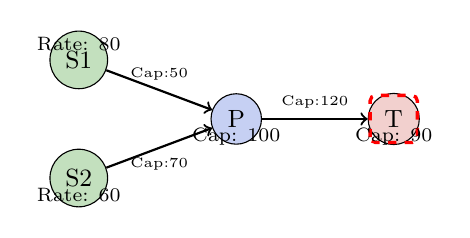
\begin{tikzpicture}[scale=1.0, font=\small]
% Nodes in compact consistent style
\node[circle, draw, fill=juliagreen!30, minimum size=0.6cm] (s1) at (0,1.5) {S1};
\node[circle, draw, fill=juliagreen!30, minimum size=0.6cm] (s2) at (0,0) {S2};
\node[circle, draw, fill=juliablue!30, minimum size=0.6cm] (p) at (2,0.75) {P};
\node[circle, draw, fill=juliared!30, minimum size=0.6cm] (t) at (4,0.75) {T};

% Edges with capacities
\draw[->, thick] (s1) -- (p) node[midway, above, font=\tiny] {Cap:50};
\draw[->, thick] (s2) -- (p) node[midway, below, font=\tiny] {Cap:70};
\draw[->, thick] (p) -- (t) node[midway, above, font=\tiny] {Cap:120};

% Bottleneck indication
\draw[red, very thick, dashed, rounded corners=2pt] (3.7,0.45) rectangle (4.3,1.05);


% Node annotations (smaller, below each node)
\node[above, font=\scriptsize] at (s1) {Rate: 80};
\node[below, font=\scriptsize] at (s2) {Rate: 60};
\node[below, font=\scriptsize] at (p) {Cap: 100};
\node[below, font=\scriptsize] at (t) {Cap: 90};
\end{tikzpicture}
\end{column}
\end{columns}

\vspace{0.3cm}
\centering

\end{frame}


\begin{frame}{The Complete IPA Toolkit}
\begin{columns}
  % Main diagram on the left
  \begin{column}{0.72\textwidth}
    \begin{center}
      \includegraphics[height=0.83\textheight]{ipa_bigpicture.png}
    \end{center}
  \end{column}

  % Utility info on the right
  \begin{column}{0.26\textwidth}
    \footnotesize
    \textbf{Access + Utilities:}
    \begin{itemize}
      \item \textbf{Visualization} tools 
      \item Input type \textbf{conversion} (CSV, JSON, GraphML)
      \item \textbf{Time unit} normalisation (mins, hours, days)
      \item Julia package (in dev) for full local use
      \item REST \textbf{API} + Angular UI deployment
      \item Lightweight web client: IPA-Web
    \end{itemize}

  \end{column}
\end{columns}
\end{frame}

\end{document}